\chapter{Introducción}


\section{Fundamentos teóricos de la luz}

\subsection{Radiación electromagnética}

La luz es radiación electromagnética que se propaga en forma de onda a través del espacio transportando energía radiante en el proceso. Está constituida por partículas elementales sin masa denominadas fotones \citep{Purcell&Morin2013}. Las propiedades de la luz están condensadas en el espectro electromagnético (EE) (Figura~\ref{espectroelectromagnetico}) con base en el número de oscilaciones de la onda por unidad de tiempo (frecuencia, $\nu$) y la distancia lineal entre dos puntos equivalentes de ondas sucesivas (longitud de onda, $\lambda$).\\

\begin{figure}
  \centering
    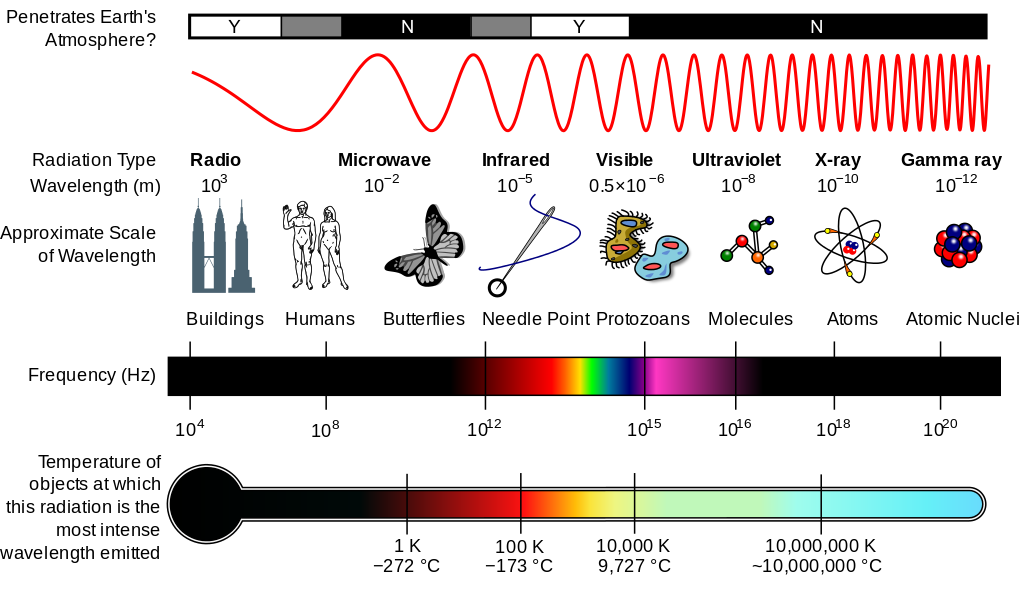
\includegraphics[width=0.9\textwidth]{espectroelectromagnetico}
  \caption{Espectro electromagnético \citep{NASA2007}}
  \label{espectroelectromagnetico}
\end{figure}

Una de las propiedades de la luz de interés para este trabajo en la región visible del EE ($\sim$ 350-800 nm) es la temperatura de color ($T$)  que está definida a partir de la Ley de desplazamiento de Wien \citep{Halliday&Resnick2008}. Esta ley explica la relación inversa entre la longitud de onda en la que se produce el pico de emisión de un cuerpo negro ($\lambda_{max}$) y $T$:

\begin{equation}
\lambda_{max} = \dfrac{b}{T}
\end{equation}

Donde $b = 2.897...\e{-3}$ m K, es denominada la constante de Wien. Un cuerpo negro es un objeto ideal que absorbe y emite toda radiación electromagnética; en equilibrio termodinámico y térmico, emite radiación térmica sólo con dependencia en su temperatura.\\

En la \textbf{\autoref{sec:luzartificial}} y en la \textbf{\autoref{sec:contaminacionluminica}} se presenta la aplicación del concepto de temperatura de color para la clasificación del color de las fuentes de luz y su implicación biológica en los humanos.\\

\subsection{Propiedades ópticas}

La óptica es el campo de la física que se encarga de estudiar la interacción de la luz con la materia. En la  \textbf{Tabla \ref{tab:propiedadesopticas}} se resumen las principales propiedades ópticas.

\begin{table}[]
\centering
\caption{Propiedades ópticas de la luz  \citep{Born&Wolf2003}}
\label{tab:propiedadesopticas}
\resizebox{0.9\textwidth}{!}{%
\begin{tabular}{|l|l|l|}
\hline
\textbf{\textbf{Propiedad}} & \textbf{} & \textbf{\textbf{Descripción}} \\ \hline
Absorción &  & La luz es captada en el objeto y aumenta su energía térmica \\ \hline
Transmisión &  & La luz atraviesa el objeto sin cambio de dirección ni intensidad \\ \hline
Dispersión &  & La luz es captada en el objeto y se re-emite con diferente dirección e intensidad \\ \cline{2-3} 
 & Rayleigh & Dispersión elástica (conserva energía) en que la longitud de onda de la luz \\
 &  & incidente es mucho mayor que el tamaño del objeto \\ \cline{2-3} 
 & \multicolumn{1}{c|} {Mie} & Dispersión elástica en que la longitud de onda de la luz incidente es similar \\
 &  & al tamaño del objeto \\ \hline
Reflexión &  & La luz se desvía al chocar con el objeto con un ángulo igual al de incidencia \\ \hline
Refracción &  & La luz cambia de dirección y velocidad al atravesar por un medio diferente \\ \hline
\end{tabular}%
}
\end{table}

\newpage

\subsection{Unidades de medición}

Existen dos campos de estudio que se encargan de la medición de la luz: la fotometría y la radiometría. La fotometría se encarga de medir la luz con base en la sensibilidad de la vista humana. Por otro lado, la radiometría mide la luz abarcando todas las longitudes de onda del EE. Al ser de carácter general este trabajo, en la \textbf{Tabla \ref{tab:unidadesradiometria}} se muestran las unidades del Sistema Internacional de Unidades (SI) utilizadas en radiometría.\\

Para estudios enfocados en los niveles de luminosidad en ecosistemas y su influencia en cada uno de sus componentes con base en su sensibilidad, es fundamental utilizar medidas fotométricas (véase el \textbf{\autoref{chap:recomendaciones}}).


\begin{table}[htb]
\centering
\caption{Unidades del SI utilizadas en radiometría \citep{Jurgen1968}}
\label{tab:unidadesradiometria}
\resizebox{\textwidth}{!}{%
\begin{tabular}{|l|l|l|}
\hline
\textbf{\textbf{Magnitud física}} & \textbf{\textbf{Unidad del SI}} & \textbf{\textbf{Notas}} \\ \hline
Energía radiante (Q) & J & Energía \\ \hline
Flujo radiante ($\Phi$) & W & Energía radiada por unidad de tiempo (potencia) \\ \hline
Intensidad radiante (I) & W sr$^{-1}$ & Potencia por ángulo sólido \\ \hline
Irradiancia (E) & W m$^{-2}$ & Potencia incidente por superficie \\ \hline
Emitancia radiante (M) & W m$^{-2}$ & Potencia emitida por superficie de la fuente radiante \\ \hline
Radiancia (L) & W sr$^{-1}$  m$^{-2}$ & Potencia por ángulo sólido y por superficie \\ \hline
Radiancia espectral ($L_{\lambda}$) & W sr$^{-1}$  m$^{-3}$ & Potencia por ángulo sólido, por superficie y por longitud de onda \\ \hline
\end{tabular}%
}
\end{table}

\newpage

\section{Brillo del cielo nocturno}
\label{sec:brillocielonocturno}

\subsection{Componentes del brillo del cielo nocturno}
\label{subsec:componentesbrillocielo}

En la \textbf{Tabla \ref{tab:componentesbrillo}} se describen los principales componentes del brillo total del cielo nocturno sin Luna $(I_{tot})$ tal como \cite{Leinert1998} lo reportan para el rango del ultravioleta lejano ($\sim$ 100 nm) al infrarrojo lejano ($\sim$ 200 $\mu$m).


\begin{table}[htb]
\centering
\caption{Componentes del brillo del cielo nocturno \citep{Leinert1998}}
\label{tab:componentesbrillo}
\resizebox{\textwidth}{!}{%
\begin{tabular}{|l|l|}
\hline
\textbf{\textbf{Componente}} & \textbf{\textbf{Descripción}} \\ \hline
Brillo del aire ($I_A$) & \begin{tabular}[c]{@{}l@{}}Excitación de átomos de oxígeno y nitrógeno de la atmósfera superior\\ por su interacción con la radiación solar\end{tabular} \\ \hline
Luz zodiacal ($I_{ZL}$) & Dispersión de la radiación solar en partículas de polvo interestelar \\ \hline
Luz estelar ($I_{ISL}$) & La luz de las estrellas en su conjunto \\ \hline
Luz difusa galáctica ($I_{DGL}$) & Luz emitida y dispersada por partículas de polvo de la galaxia \\ \hline
Luz de fondo extragaláctica ($I_{EBL}$) & Luz producida por galaxias o cúmulo de galaxias \\ \hline
Luz artificial ($I_{SCA}$) & Luz artificial dispersada en la tropósfera \\ \hline
\end{tabular}%
}
\end{table}

La suma de tales componentes (excepto luz artificial, netamente de origen antropogénico) se considera de origen natural y es susceptible de ser atenuada por acción de la atenuación atmosférica. De acuerdo con esta clasificación, el brillo total del cielo nocturno puede calcularse a partir de la siguiente ecuación:

\begin{equation}
I_{tot} = (I_A + I_{ZL} + I_{ISL} + I_{DGL} + I_{EBL})\:e^{-\tau} + I_{SCA}
\end{equation}

\vspace{2mm} 

Donde $\tau$ es el coeficiente de atenuación atmosférica que depende de la longitud de onda, la distancia cenital (la distancia angular del cuerpo celeste con respecto al cenit), la altura sobre el nivel del mar del observador y las condiciones atmosféricas.\\ 

La definición matemática del brillo total del cielo nocturno nos permite inferir que las principales contribuciones se deben al brillo del aire y a la luz zodiacal; estimaciones experimentales confirman este comportamiento reportando mediciones de radiancia de hasta 10$^{-4}$ W sr$^{-1}$  m$^{-2}$ atribuibles al brillo del aire \citep{Leinert1998}.\\ 

\subsection{Variación natural del brillo del cielo nocturno por influencia de la Luna}

La luz lunar percibida en la Tierra es resultado de la reflexión de la luz solar y, en menor medida, terrestre en la superficie de la Luna. El albedo lunar es 0.136 lo que significa que refleja 13.6\% del total de la radiación incidente \citep{Matthews2008}. La cantidad de luz lunar varía hasta en tres órdenes de magnitud a lo largo del mes de acuerdo con el ciclo lunar \citep{Kyba2017}.\\

En condiciones atmosféricas despejadas y de nula luz artificial, la luz lunar es la principal responsable del brillo total del cielo nocturno ya que, típicamente, los valores de brillo del aire son hasta tres órdenes de magnitud más pequeños que los reportados para la luz lunar \citep{Hanel2018}.\\

\newpage

Es importante tomar en cuenta la advertencia de \cite{Kyba2017} quienes reportan que en la literatura científica existen datos erróneos de luz lunar y hacen visible la necesidad de una publicación que reporte valores típicos de referencia de luz lunar a través de estudios de largo plazo (al menos de un año) en localidades sin influencia de luz artificial.\\ 

Tomando en cuenta las consideraciones anteriores, para efectos de este estudio centrado en la luz artificial, se procede a despreciar los términos de luz de origen natural en la ecuación de brillo total del cielo nocturno sin Luna, reduciéndose entonces a:

\begin{equation}
I_{tot} = I_{SCA}
\end{equation}\\


\subsection{Variación natural del brillo artificial del cielo nocturno por influencia de las condiciones atmosféricas}

\subsubsection{Propiedades ópticas del aerosol atmosférico}
\label{subsubsec:propiedadesopticasaerosol}


La concentración de aerosol atmosférico depende principalmente de emisiones naturales y antropogénicas, patrones de circulación sinóptica, meteorología local y características topográficas \citep{Carabali2017}.\\

\cite{Garstang1991} describió por primera vez la dispersión de la luz artificial por acción del aerosol atmosférico. Posteriormente \cite{Kocifaj2007} verifica que el aerosol atmosférico puede amplificar o reducir el brillo del cielo nocturno con base en las propiedades ópticas de bulto descritas a continuación.\\

\textit{\textbf{Espesor óptico de aerosol (AOD)}}\\

El AOD es una cantidad adimensional que representa la atenuación atmosférica de la luz por el aerosol atmosférico integrada verticalmente en toda la columna atmosférica. La diferencia de potencial ($V$) medido por un fotómetro solar es proporcional a la radiancia espectral ($L_{\lambda}$) que es captada por el instrumento en la superficie \citep{Holben1998}. El espesor óptico total ($\tau_{TOT}$) puede calcularse a partir de la siguiente ecuación conocida como la ley de Beer-Lambert-Bouguer:

\begin{equation}
V(\lambda) = V_0(\lambda)\:d^{2} \:e^{-\tau_{TOT}\: m}
\end{equation}

Donde $V$ es la diferencia potencial medida en una longitud de onda dada $\lambda$, $d$ es la tasa entre el promedio y la distancia real Tierra-Sol y $m$ es la masa óptica de aire. La masa óptica de aire es la tasa entre la masa de aire que la luz solar atraviesa hasta la superficie de la Tierra y la masa de aire que atravesaría si la incidencia fuera vertical.\\

Otros constituyentes atmosféricos pueden dispersar la luz y, por lo tanto, deben de considerarse en el cálculo del AOD \citep{Holben1998} tal y como se muestra en la siguiente ecuación:

\begin{equation}
\tau (\lambda)_{Aerosol} = \tau (\lambda)_{TOT} - \tau (\lambda)_{agua} - \tau (\lambda)_{Rayleigh} - \tau (\lambda)_{O_3} - \tau (\lambda)_{NO_2} - \tau (\lambda)_{CO_2} - \tau (\lambda)_{CH_4}
\end{equation}

\newpage

\textit{\textbf{Parámetro de Angstrom}}\\

La distribución por tamaño del aerosol atmosférico puede ser estimada a través del Parámetro de Angstrom $(\alpha)$ \citep{Holben1998} definido a partir de la siguiente ecuación:

\begin{equation}
\alpha (\lambda_1, \lambda_2) = \frac { -ln (\frac{\tau_\lambda_2}{\tau_\lambda_1})}{ ln(\frac{\lambda_2}{\lambda_1})}
\end{equation}

Donde $\tau_\lambda_1$ y $\tau_\lambda_2$ son el AOD en las longitudes de onda $\lambda_1$ y $\lambda_2$ respectivamente. Típicamente los valores de $\alpha$ varían entre -2 y 2.  $\alpha$ $>$ 1, indica que el modo fino de aerosol atmosférico es dominante mientras que  $\alpha$ $<$ 1 indica que el modo grueso es el más abundante \citep{Carabali2017}.\\

\textit{\textbf{Parámetro de Asimetría (ASY)}}\\

Su valor es una medida de la dirección de la dispersión de la luz. Está definido como el promedio del coseno del ángulo de dispersión $\theta$ ponderado por intensidad de la luz:

\begin{equation}
ASY = < cos \theta > = \frac{1}{2} \int_{0}^{\pi} sen (\theta) cos(\theta) P(\theta) d\theta
\end{equation}

Con $P(\theta)$ la función de fase de dispersión que describe la dispersión de la luz dependiente del ángulo:

\begin{equation}
P(\theta) = \frac{4\pi}{\sigma_{SCA}} \frac{d\sigma_{SCA}}{d\theta}
\end{equation}

Donde $\sigma_{SCA}$ es la sección transversal de dispersión:

\begin{equation}
\sigma_{SCA} = \frac{\pi D^{2}}{4} Q_{SCA}
\end{equation}

Con $D$ el diámetro de la partícula y $Q_{SCA}$ la eficiencia de dispersión (cuánta energía absorbida es dispersada).\\

Cuando ASY = 1, toda la luz es dispersada hacia adelante; ASY = 0, indica una dispersión isotrópica \citep{Solano2015}.
\\

\textit{\textbf{Albedo de Dispersión Simple (SSA)}}\\

Este parámetro relaciona los coeficientes de dispersión ($\epsilon_{SCA}$) y absorción ($\epsilon_{ABS}$) \citep{Foot1987} como muestra la ecuación:

\begin{equation}
SSA = \frac{\epsilon_{SCA}}{\epsilon_{SCA} + \epsilon_{ABS}}
\end{equation}


Los coeficientes de dispersión $\epsilon$ se obtienen:

\begin{equation}
\epsilon = N \sigma
\end{equation}

Con $N$ la concentración de partículas de tamaño $D$. El valor del SSA es representativo de las propiedades de absorción de la luz del aerosol atmosférico. Cuando el valor del SSA es cercano a 1 es un indicativo que el aerosol en cuestión refleja más luz, mientras que, para el aerosol más absorbente, el valor del SSA es cercano a 0.\\

\subsubsection{Propiedades ópticas de las nubes}

\cite{Twomey1967} desarrolló por primera vez una teoría de dispersión de la luz debido a la nubosidad. Estudios más recientes \citep{Kocifaj2007}, \citep{Solano2014}, \citep{Solano2015}, han encontrado cambios significativos en el brillo del cielo por la dispersión de luz artificial por acción de la nubosidad. Las nubes son un medio dispersivo complejo, esto es, que poseen diferentes constituyentes con diferente índice refractivo complejo $(\underline{n})$ definido como:

\begin{equation}
\underline{n} = n + i k
\end{equation}

\vspace{2mm} 

Donde $n$, la parte real de la ecuación, indica la velocidad de la luz dentro de un medio y la parte imaginaria $k$ es el coeficiente de atenuación de la luz dentro del medio en cuestión \citep{Born&Wolf2003}. Los valores de la parte imaginaria del índice refractivo complejo para las gotitas de nube y los cristales de hielo que forman las nubes son muy bajos de acuerdo con \cite{Solano2015}.\\

Tomando en cuenta lo anterior, \cite{Solano2015} consideran a las nubes como cuerpos Lambertianos con albedo espectral variante para su estudio óptico. Un cuerpo Lambertiano es aquel que posee una superficie ideal que refleja la luz incidente de manera isotrópica, permitiendo así que el brillo de tal superficie sea la misma para el observador independientemente de su ángulo de visión \citep{Born&Wolf2003}.\\

El albedo espectral de las nubes depende principalmente de factores como la altitud de su base con respecto al observador y la microfísica incluyendo el contenido de agua líquida y la distribución por tamaño de las gotitas de nube \citep{Kocifaj2007}.\\ 

Resulta complicado medir el albedo espectral de las nubes durante la noche ya que la mayoría de los fotómetros que miden esta propiedad funcionan con base en niveles de radiación presentes sólo durante el día. Por esta razón, las simulaciones numéricas de la influencia de las nubes en el brillo del cielo nocturna resultan útiles \citep{Solano2015}.\\

Además, es importante mencionar que los factores que se toman en cuenta en la modelación teórica son capaces de reproducir diferentes comportamientos del brillo del cielo con respecto a la posición del observador, lo cual es deseable para la predicción del brillo del cielo nocturno influenciado por diferentes tipos de nubes \citep{Kocifaj2007}, \citep{Solano2015}.

\newpage

\section{Luz artificial}\\
\label{sec:luzartificial}

En esta sección se aborda la caracterización de la luz artificial (de origen netamente antropogénico). Para esta tesis se considera que el alumbrado público es el principal responsable del brillo del cielo nocturno ocasionado por luz artificial \citep{Solano2013b}.

\subsection{Fundamentos teóricos de las fuentes artificiales de luz}

El diseño de iluminación es una disciplina fundamental para la correcta iluminación en el alumbrado público, la cual requiere de colaboraciones con otros campos como la física, biología, ciencias de la Tierra, ingeniería y arquitectura. El reto es grande ya que una correcta iluminación debe ser sustentable, apropiada para su contexto y debe lograr ahorro económico \citep{LibroCL}, \citep{Globaldiscussion}. A continuación se presentan los conceptos físicos fundamentales detrás de la iluminación.\\


\textbf{Producción de luz}

Para la producción artificial de luz se necesita de una serie de transformaciones de energía. El primer paso es la generación de energía eléctrica. De acuerdo con \cite{Ramos2012}, la mayoría de la energía eléctrica consumida en México es generada a partir de la transformación de energía química por medio de la combustión de hidrocarburos.\\

Una vez generada la energía eléctrica, necesita ser transformada en energía radiante. Esto se logra por medio del mecanismo interno de la fuente de luz. Los mecanismos más utilizados son la termorradiación (radiación de un cuerpo caliente) y luminiscencia (radiación de cuerpo no caliente) \citep{LibroCL}. En la \textbf{\autoref{subsec:fuentesdeluz}} se abordan las particularidades de cada uno de estos mecanismos.\\


\textbf{Distribución espectral}

La cantidad de energía radiada en determinadas regiones del EE \citep{Solano2013}. En la \textbf{\autoref{subsec:fuentesdeluz}} se muestran los gráficos de distribución espectral para diferentes tipos de fuentes de luz artificial.\\

  
\textbf{Temperatura de color}

La temperatura de color define el color de una fuente de luz sólo si esta se asemeja a un cuerpo negro. La mayoría de las fuentes de luz tradicionalmente utilizadas (incandescentes) se asemejan a un cuerpo negro, mientras que para las que no cumplen con esa característica (de descarga y LED), se implementa la temperatura de color correlacionada \citep{LibroCL}.\\

Para efectos de evaluación de reproducción de color y confort se asocia una apariencia de color a los rangos de temperatura de color teniendo <<luz cálida>> para temperatura de color de hasta 3000 K, <<luz intermedia>> de 3000 - 5300 K y <<luz fría>> para temperaturas de color mayor a 5300 K \citep{Globaldiscussion}.\\


\textbf{Eficiencia}

Definida para estudios fotométricos, se trata de la cantidad de flujo luminoso (visible) emitido por una fuente de luz por unidad de potencia consumida. La unidad del flujo luminoso es el lumen (lm), el equivalente fotométrico del flujo radiante. No es posible obtener una eficiencia de 100$\%$ debido a las pérdidas ocasionadas por disipación calorífica y radiaciones no visibles para el humano \citep{LibroCL}.


\subsection{Fuentes de luz artificial}
\label{subsec:fuentesdeluz}

Existen tres principales tipos de fuentes de luz artificial: incandescente, de descarga y diodo emisor de luz (LED, por sus siglas en inglés) (\textbf{Tabla \ref{tab:luzartificial}}), (Figura~\ref{distribucionespectral})  \citep{Solano2013b}, \citep{Eldvidge2010}, \citep{LibroCL}.\\

La iluminación incandescente es la más antigua y la más utilizada para interiores, su funcionamiento se basa en hacer pasar corriente eléctrica a través de un filamento, aumentando su temperatura hasta hacer que emita radiaciones visibles (termorradiación).\\

Por otro lado, la luz de descarga, utilizada ampliamente para alumbrado público, es generada por la excitación de un gas sometido a descargas eléctricas entre dos electrodos (luminiscencia).\\

Por último, el LED, que recientemente se ha comenzando a implementar en el alumbrado público, genera luz moviendo electrones de un semi-conductor sólido de un estado de alto nivel de energía a uno más bajo a través de la aplicación de una diferencia de potencial (electroluminiscencia).


\begin{table}[htb]
\centering
\caption{Principales fuentes de luz artificial}
\label{tab:luzartificial}
\resizebox{\textwidth}{!}{%
\begin{tabular}{|c|c|c|c|}
\hline
\textbf{Tipo} & \textbf{Fuente de luz} & \textbf{Temperatura de color (K)} & \textbf{Eficiencia (lm W$^{-1}$)} \\ \hline
Incandescente & Lámpara incandescente & 2700 & 8 - 18 (baja) \\ \hline
De descarga & Lámpara de sodio a baja presión (LPS) & 2000 & 180 (muy alta) \\ \cline{2-4} 
 & Lámpara de sodio a alta presión (HPS) & 2300 & 100 (alta) \\ \cline{2-4} 
 & Lámpara de halogenuros metálicos (MH) & 2800 - 5000 & 70 - 90 (alta) \\ \cline{2-4} 
 & Lámpara de vapor de mercurio (MV) & 3200 - 4000 & 60 (media) \\ \hline
LED & LED & 2700 - 5000 & 10 - 150 (baja) \\ \hline
\end{tabular}%
}
\end{table}


\begin{figure}[htb]
  \centering
    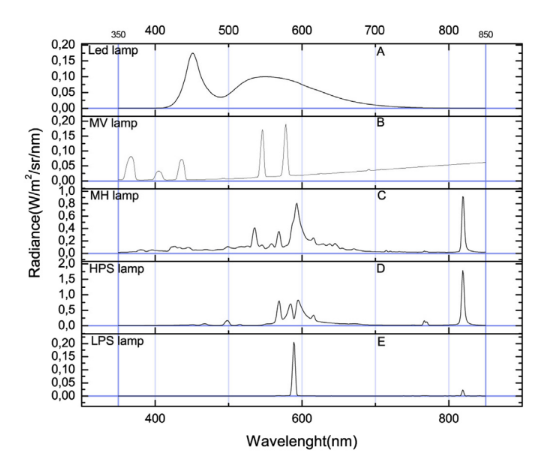
\includegraphics[width=100mm, scale=1]{distribucionespectral}
  \caption{Distribución espectral de A) LED, B) Vapor de mercurio, C) Halogenuros metálicos, D) Sodio a alta presión y E) Sodio a baja presión \citep{Solano2013b}}
  \label{distribucionespectral}
\end{figure}

\newpage

\subsection{Tipos de luminarias}
\label{subsec:luminarias}

Las luminarias son dispositivos que alojan y protegen la fuente de luz y reconducen su luz hacia donde se quiere iluminar \citep{LibroCL}. Para el caso del alumbrado público existen dos tipos: luminarias para vías principales (autopistas, carreteras) y luminarias para vías secundarias (calles) \citep{INFO2019}.\\

La forma en que la luminaria distribuye en el espacio la luz emitida por la fuente es fundamental en el efecto sobre el brillo del cielo nocturno. \cite{Marin2009} propone el ángulo entre la línea vertical de la fuente de luz y la línea máxima a la que ilumina (ángulo de apantallamiento) para garantizar un buen aprovechamiento de la luz y evitar que se desperdicie escapando hacia la atmósfera. El ángulo de apantallamiento ideal es por debajo de los 75\grad (A); para ángulos mayores a ese (B - E) existe afectación en diferente proporción al brillo del cielo nocturno (Figura~\ref{anguloapantallamiento}).


\begin{figure}[htb]
  \centering
    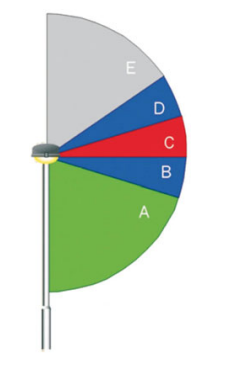
\includegraphics[width=30mm, scale=0.3]{anguloapantallamiento}
  \caption{Ángulo de apantallamiento de luminaria \citep{Marin2009}}
  \label{anguloapantallamiento}
\end{figure}


\subsection{Función de emisión urbana}
\label{subsec:funciondemisionurbana}

Las fuentes de luz artificiales (públicas y privadas) emiten luz en casi todas las direcciones \citep{Kocifaj2014}, \citep{Kocifaj2016}. Por lo tanto, la luz artificial emitida a la atmósfera se debe a la superposición de emisiones de las diferentes fuentes distribuidas en la superficie.\\

La distribución angular de la luz emitida por una ciudad es fundamental para la modelación del brillo del cielo nocturno ocasionado por luz artificial \citep{Kocifaj2014} esta distribución es caracterizada a través de una función de emisión parametrizada denominada Función de Emisión Urbana (CEF, por sus siglas en inglés) la cual depende de las características del sistema de iluminación de una ciudad \citep{Kocifaj2014}.\\

Debido a la falta, hasta la actualidad, de inventarios detallados de las fuentes de luz (públicas y privadas) y su naturaleza heterogénea, resulta extremadamente complicado obtener la CEF a través de estudios teóricos o experimentales \citep{Kocifaj2014}. \cite{Garstang1986} desarolló una aproximación semi-empírica para la estimación de la CEF, la cual es discutida en el \textbf{\autoref{chap:metodologia}}

\newpage

\section{Contaminación lumínica (CL)}\\
\label{sec:contaminacionluminica}

La CL es cualquier efecto negativo debido a la emisión de luz artificial en intensidades, direcciones, rangos espectrales u horarios innecesarios \citep{AtlasREPSA}, \citep{LibroCL}, \citep{Stone2017}.\\

En esta sección se presentan los argumentos que permiten afirmar que el brillo del cielo nocturno ocasionado por la luz artificial, es una fuente de CL en los socioecosistemas. Entiéndase contaminación como la alteración negativa de un sistema a través de la introducción de elementos físicos extraños \citep{AtlasREPSA}, \citep{LibroCL}.\\

Entiéndase un sistema como un conjunto de componentes interactuando en los que: 1) el comportamiento de cada componente tiene un efecto en el comportamiento del todo y, 2) el comportamiento de los componentes y sus efectos en el todo son interdependientes \citep{Avila2019}.\\

\subsection{El enfoque socioecosistémico}

Los seres humanos nombramos a la realidad natural de distintas maneras, las cuales poseen significados brutalmente diferentes de acuerdo con el fundamento filosófico con el que percibimos el planeta \citep{Avila2019}, \citep{Uribe2014}. Por ejemplo, las empresas extractivas denominan <<recursos naturales>> a tal realidad, los habitantes de una región, <<territorio>> y los científicos, <<ecosistema>>.\\

Con la aparición de la vida en la Tierra, surgieron los ecosistemas como un nivel de organización de la materia y la energía, en que el los sistemas físico-químicos (abióticos) y los sistemas bióticos interctuaron y evolucionaron de manera integrada. Sin embargo, con la emergencia de las sociedades y su organización con base en un lenguaje simbólico, nacen los socioecosistemas \citep{Avila2019}, \citep{Uribe2014}, \citep{Urquiza2015}.\\

Un socioecosistema es, por lo tanto, un sistema complejo (no lineal) y adaptativo que hace referencia a los procesos de acoplamiento e interacción entre los sistemas sociales (cultura, economía, organización social y política) y los ecosistemas \citep{Urquiza2015}.\\

Resulta fundamental, entonces, estudiar las problemáticas de contaminación ambiental desde el enfoque socioecosistémico. De esta manera se hace visible que, separar el nicho humano de la realidad natural, es el principal motor de la actual crisis ambiental. En este sentido, las Ciencias de la Tierra surgen como la disciplina integradora que, a través de la generación de conocimiento con un enfoque socioecosistémico, logra sembrar directrices en la construcción de la sustentabilidad.\\

\subsection{Importancia del ciclo día-noche en la evolución de la vida}

La duración del ciclo día-noche en la Tierra ha cambiado significativamente a lo largo de la historia geológica debido a la variación de la velocidad de rotación del planeta. La velocidad de rotación original de los planetas  es consecuencia de la conservación del momento angular que poseía la nebulosa interestelar que, al colapsar, dio origen al Sistema Solar hace aproximadamente 4600 Ma \citep{Greaves2005}.\\

Sin embargo, si la hipótesis del Impacto de Theia es correcta, es factible que la rotación primordial de la Tierra haya sido reconfigurada hace alrededor de 4500 Ma, cuando un cuerpo astronómico del tamaño de Marte, nombrado Theia, colisionó tangencialmente con nuestro planeta dando origen, además, a la Luna \citep{Stevenson1987}.\\

La velocidad de rotación actual de la Tierra debió comenzarse a perfilar hacia finales del periodo Criogénico (hace alrededor de 600 Ma), al mismo tiempo que los niveles de oxígeno y ozono estratosférico fueron óptimos para el surgimiento y desarrollo de vida más compleja (multicelular) en un evento conocido como \textit{la Radiación del Cámbrico}, durante el que se originaron y diversificaron la mayoría de los filos animales incluyendo el de los cordados, al que pertenecemos los humanos \citep{Conway2000}.\\

La mayoría de los organismos, incluyendo a los humanos, poseen ritmos circadianos que son controlados por el ciclo día-noche. Tales ritmos juegan un papel primordial en la regulación del metabolismo, el crecimiento y el comportamiento \citep{Dunlap1999}. Los fotoreceptores circadianos han estado presentes en la retina de los vertebrados desde hace aproximadamente 500 Ma, una vez que la duración del día se estableció en 24 horas \citep{Conway2000}, \citep{Longcore2006}.\\

Se ha encontrado que la proporción de especies vertebradas nocturnas que surgieron durante radiaciones evolutivas recientes es mayor con respecto a las antiguas (Figura~\ref{nocturnalidad}). Esto sugiere que la nocturnalidad es un importante paso en la evolución de los vertebrados \citep{Holker2010}. Sin embargo, no sólo la nocturnalidad es importante en los vertebrados, se estima que más del 60$\%$ de invertebrados son nocturnos \citep{Longcore2006}.


\begin{figure}[htb]
  \centering
    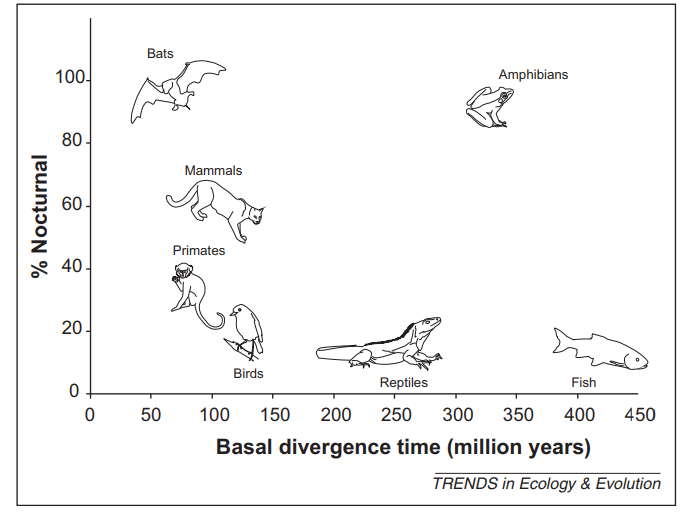
\includegraphics[width=95mm, scale=0.95]{nocturnalidad}
  \caption{Porcentaje de especies nocturnas de diferentes clases y órdenes de vertebrados con respecto a su origen \citep{Holker2010}}
  \label{nocturnalidad}
\end{figure}

Se teoriza que dada la alta permeabilidad de la piel de los anfibios y por ende, la susceptibilidad a las características de los nichos diurnos como la radiación solar, estos tuvieron que adoptar la nocturnalidad tempranamente \citep{Holker2010}.

\newpage

\subsection{Breve historia del uso y abuso de la luz artificial}\\
\\

Es sabido que el control regular del fuego por nuestros antepasados, desde hace aproximadamente 400 ka \citep{Dunbar2014}, fue fundamental en la evolución humana: la capacidad de cocinar alimentos mejoró la digestión y aprovechamiento de calorías, generando así el aumento de la masa cerebral; la llamas del fuego proveyeron protección de los predadores, permitiendo a los primeros humanos extender sus nichos ecológicos \citep{Wrangham2010}.\\

Por otro lado, la luz artificial del fuego extendió por primera vez la duración del día para las primeras sociedades. Las actividades nocturnas estuvieron lejos de ser económicamente productivas (exclusivamente diurnas); tales horas extras se dedicaron al canto, el baile, las ceremonias religiosas y a contar historias, lo que provocó una alteración en los ritmos circadianos de los primeros humanos \citep{Wiessner2014}.\\

Mientras que la observación de la Luna y las estrellas despertó el sentido de vulnerabilidad y preguntas sobre el origen del universo, las historias nocturnas crearon un espacio y contexto propicio para desarrollar órdenes más complejos de la conciencia de sí mismo, el entendimiento de los pensamientos y sentimientos de los otros, y la generación, regulación y transmisión de instituciones culturales \citep{Wiessner2014}.\\

Un esquema similar al de las primeras sociedades se siguió en los grupos humanos antiguos: los griegos, egipcios y chinos utilizaron lámparas de aceite en contextos religiosos a principios de la era común. Hasta antes de la Revolución Industrial (mediados del siglo XVIII) se utilizaron velas de cera y sebo con fines no económicos: como fuente de calor y fragancia e incluso para la cuenta del tiempo \citep{Duvall1988}.\\

Con la llegada de la Revolución Industrial como antecedente del capitalismo, los valores en torno a la luz artificial cambiaron radicalmente: la luz eléctrica se hizo necesaria para la iluminación de las jornadas nocturnas y el regreso a casa de los trabajadores. Se comenzaron a extender las horas productivas tradicionalmente restringidas durante el día para aumentar la producción \citep{Hudson1992}. Es fácil seguir esta tendencia hasta nuestros días al revisar las estadísticas que muestran que la mayor parte de energía eléctrica es utilizada para la industria y alumbrado público/privado \citep{Ramos2012}.\\ 


En conclusión, la lógica capitalista bajo la que vivimos ha transformado las horas nocturnas dedicadas antiguamente al descanso y a la realización de actividades espirituales y culturales en tiempo económicamente productivo gracias a la luz artificial producida e implementada en gran escala la cual, aún peor, está muy lejos de ser sustentable (véase \textbf{\autoref{subsec:consecuenciascl}} y \textbf{\autoref{subsec:consumoenergiaelectrica}}).

\newpage

\subsection{Tipos de CL} 

Hasta este punto únicamente se ha mencionado el brillo del cielo nocturno (objeto de este estudio) como un tipo de CL, sin embargo existen otros tipos \citep{LibroCL} los cuales es importante mencionar y se abordan a continuación.\\ 

\textbf{Emisión directa}

Es la emisión procedente directamente de la fuente de luz hacia el entorno originalmente oscuro. Es la causa más crítica de contaminación, debido a la intensidad de la fuente.\\ 

\textbf{Luz reflejada}

La luz es reflejada en el suelo o construcciones en direcciones no deseadas.\\ 


De acuerdo con el Nuevo Atlas Mundial del Brillo Artificial del Cielo Nocturno \citep{Falchi2016} aproximadamente 80$\%$ de la población mundial vive bajo algún tipo de CL, siendo el brillo del cielo nocturno el tipo más extendido.\\ 

En conclusión, la energía radiante del alumbrado público y privado es la causa de la CL y mientras esté funcionando durante la noche, la CL será inevitable. Sin embargo sus consecuencias pueden ser reducidas considerablemente, eliminando la emisión directa y regulando la luz reflejada y el brillo del cielo nocturno.\\ 

\subsection{Consecuencias de la CL}
\label{subsec:consecuenciascl}

Regularmente al alumbrado público y privado se les denota de una manera positiva asignándoles valores asociados con la seguridad, estética e identidad los cuales, desafortunadamente, al ser abordados de manera no sustentable invisibilizan el <<lado oscuro de la luz>> que se aborda en la presente subsección \citep{Globaldiscussion}, \citep{LibroCL}.\\ 

Las consecuencias de la CL son extremadamente diversas y afectan en diferentes escalas a los socioecosistemas. Sin embargo, basta con remitirse a la definición de CL para entender, a grandes rasgos las relaciones causa-consecuencia. Esto es, la luz artificial se vuelve contaminante cuando es emitida en intensidades, direcciones, rangos espectrales, horarios innecesarios o en cualquier combinación de estas características \citep{AtlasREPSA}, \citep{LibroCL}, \citep{Stone2017}.\\ 

A continuación se mencionan algunas de las consecuencias de la CL clasificadas de acuerdo con su afectación en los socioecosistemas (de manera directa e indirecta). Este recuento no pretende ser exhaustivo pero sí ser representativo de las consecuencias más apremiantes y cuyo estudio es todavía emergente.\\

\textbf{Consecuencias directas}\\ 

Hasta este punto únicamente se ha mencionado la temperatura de color como indicador de confort en los humanos. Sin embargo, esta propiedad al ser cualitativa no es suficiente para evaluar el impacto de la CL en diferentes especies. Para tales fines resulta necesario basarse en el espectro de emisión de las fuentes de luz \citep{CEI2017}.\\

\newpage

Como todas las fuentes de luz de amplio espectro, los LEDs producen una porción de su radiación en longitudes de onda cortas (véase la Figura~\ref{distribucionespectral}). Debido a que las las radiaciones con longitud de onda corta se dispersan con mayor facilidad en la atmósfera terrestre que las de longitud de onda larga y que, además, se ha encontrado marcada sensibilidad biológica a las longitudes de onda corta, se ha planteado que los LEDs son una de las fuentes de luz con mayor potencial en términos de CL \citep{USENERGY2017}.\\

Sin embargo, también es necesario mencionar que los efectos adversos que puedan generar las radiaciones tanto de longitud de onda corta, como de longitud de onda larga, dependen de otros factores tales como la intensidad y el tiempo de exposición \citep{Globaldiscussion}. Dentro de las consecuencias directas de la CL en diferentes tipos de seres vivos se cuentan las siguientes:\\


\textit{\textbf{Insectos}}\\

Los insectos son los principales invertebrados afectados por la CL ya que su actividad es básicamente nocturna. Utilizan  la luz del firmamento como referencia de navegación y sus sistemas visuales están adaptados a niveles muy bajos de luz. Los efectos de la CL en los insectos principalmente son la captación (muerte por impacto o agotamiento al ser atraídos a las fuentes de luz artificial), pérdida de visión, desorientación en la navegación y alteración de conductas reproductivas (la luz puede suprimir la emisión de feromonas o dificultar la actividad de atracción) \citep{CEI2017}, \citep{Davies2013}.\\

\textit{\textbf{Anfibios}}\\

Como se comentó con anterioridad, los anfibios son los vertebrados más afectados por la CL. Su tegumento (tejido orgánico que cubre su cuerpo) es altamente glandular, carece de protección contra la radiación ultravioleta, y es sensible a la luz y al calor. La CL también tiene efecto sobre su reproducción (la luz inhibe los llamados de atracción), retrasos en el crecimiento y variación en el comportamiento de caza (migración de especies a lugares iluminados donde hay mayor densidad de insectos, lo cual los hace más vulnerables a las condiciones del entorno) \citep{Longcore2006}, \citep{LibroCL}, \citep{LibroCL}.\\

\textit{\textbf{Aves}}\\

La CL afecta especialmente la migración de las aves: las luces de edificios iluminados desorientan la navegación y dificultan la ocultación de predadores \citep{Longcore2006}.\\

\textit{\textbf{Mamíferos}}\\

La mayor afectación de la CL en los mamíferos es en la alteración de los ritmos circadianos, que como se mencionó con anteriordad, su funcionamiento está totalmente supeditado al ciclo día-noche y son fundamentales en la regulación del metabolismo, el crecimiento y el comportamiento.\\

En este punto resulta importante mencionar los efectos en la salud humana debido a la CL. La alteración en los ritmos circadianos humanos se asocia con la supresión de la producción de la hormonas que sólo se producen durante total oscuridad como la melatonina. Se ha reportado que el déficit de melatonina y la disrupción circadiana en general, están asociadas con un gran número de patologías entre otras el aumento de la incidencia del síndrome metabólico, enfermedades cardiovasculares, alteraciones cognitivas y afectivas, riesgo de padecimiento de algunos tipos de cáncer y envejecimiento prematuro \citep{CEI2017}, \citep{LibroCL}.\\

Debido a los orígenes multifactoriales de las patologías anteriormente descritas, hasta el momento, no es posible asociar directamente la CL como causante de tales. Sin embargo, las patologías oculares como las retinopatías sí pueden deberse en gran medida la exposición a luz intensa y luz con longitudes de onda cortas \citep{CEI2017}.\\


\textbf{Consecuencias indirectas}\\ 

En este tipo de consecuencias se hace aún más evidente la falta de sustentabilidad en la iluminación artificial de las ciudades. Además de afectar directamente la salud de los componentes biológicos de los socioecosistemas, la CL compromete la continuidad de los sistemas físicos (base de los componentes biológicos y sociales de los socioecosistemas). Las principales afectaciones en este sentido son la pérdida de los cielos oscuros, el derroche energético (y por consiguiente económico), sinergia con el cambio climático y la contaminación atmósfera.\\ 


\textit{\textbf{Pérdida de los cielos oscuros}}\\ 

La pérdida de los cielos oscuros debido a la CL no sólo afecta a la astronomía; valores éticos y espirituales que generalmente son minimizados en el estudio de la CL están siendo comprometidos. \cite{Stone2017} aborda estos valores a través de su categorización en <<conexión con la naturaleza>>, <<visibilidad de las estrellas>>, <<patrimonio y tradición>> y <<maravilla y belleza>>.\\ 


\textit{\textbf{Derroche energético}}\\ 

El derroche energético que se genera a raíz de la CL tiene implicación en la emisión de Gases de Efecto Invernadero (GEI) y, por lo tanto, en el calentamiento global. Tal implicación es tan alta que, de acuerdo con \cite{Gallaway2010}, si se eliminara toda la luz artificial desperdiciada en Estados Unidos ocurriría un efecto equivalente en las emisiones de CO$_{2}$ que si removieran 9.5 millones de automóviles de circulación. Desde esta perspectiva, el proteger los cielos oscuros es también una manera de exigir un uso sustentable de la energía y mitigar el cambio climático.\\ 

\textit{\textbf{Contaminación atmosférica}}\\ 

Un aspecto interesante es el que sugiere que la luz artificial durante la noche podría producir un efecto sinérgico en la contaminación atmosférica al funcionar como un potencial estímulo de nucleación de partículas ultrafinas (peligrosas para el sistema respiratorio) y contaminantes como el ozono que, entre otros factores, se forman a partir de reacciones fotoquímicas \citep{LibroCL}.\\ 

\newpage 
 
\subsection{Estudio de la CL}

La necesidad de cuantificar continuamente la CL ha propiciado el desarrollo de herramientas experimentales (instrumentos de medición) y teóricas (modelos) \citep{Kocifaj2015}. Sin embargo, la mayoría de los instrumentos que miden el brillo del cielo nocturno suelen tener limitaciones que dificultan la obtención e interpretación de los datos.\\

El instrumento más utilizado para medir el brillo del cielo nocturno es el Sky Quality Meter (SQM), este equipo únicamente es capaz de hacer mediciones puntuales en el cenit, lo cual no es representativo de la distribución angular de la radiancia en el cielo \citep{Ribas2015}. Por otro lado, los instrumentos de interés (incluido el SQM) están diseñados para medir en regiones específicas del EE, lo que implica una pérdida de información valiosa \citep{Ribas2015}.\\

Ademas de compensar las deficiencias presentes en los instrumentos de medición, los modelos han resultado adecuados para la construcción de simulaciones significativamente estadísticas de distribución de luz en el cielo nocturno las cuales poseen fundamentos teóricos robustos con significado físico \citep{Solano2015}.\\

Los primeros intentos de desarrollar una ley de propagación de la luz en el cielo nocturno surgieron después de que la CL comenzó a significar un problema para la comunidad astronómica. En este sentido \cite{Bertiau1973} presentaron un modelo simplificado que estimaba el brillo artificial cenital a través de la función población - brillo $F (D)$ y la función brillo - distancia $Q (D)$ de las ciudades aledañas \citep{Linares2018}.\\

Un paso importante hacia un modelo más completo lo dio \cite{Garstang1986} quien en lugar de considerar las ciudades como fuentes puntuales, las modeló como superficies circulares uniformes \citep{Linares2018} y, como se menciona en la \textbf{\autoref{sec:brillocielonocturno}} y en la \textbf{\autoref{sec:luzartificial}}, la cantidad de aerosol atmosférico es un parámetro ajustable e incluye la reflectancia del suelo y el porcentaje de luz emitida hacia la atmósfera a través de la Función de Emisión Urbana.\\

Hoy en día existen dos modelos prominentes: \textit{SkyGlow} \citep{Kocifaj2007} e \textit{ILLUMINA} \citep{Aube2005}. Ambos modelos consideran la distribución heterogénea de las fuentes de luz. \textit{SkyGlow} sólo toma en cuenta dispersión de primer orden, lo que lo hace adecuado para observadores cercanos a las fuentes de luz mientras que \textit{ILLUMINA} incluye dispersión de primer y segundo orden, lo que permite experimentos en cualquier dirección y distancia (lo que requiere mayor tiempo computacional con respecto a \textit{SkyGlow}) \citep{Linares2018}. Por esta razón \textit{SkyGlow} es recomendable para experimentos que incluyen una malla con gran número de puntos (dominio geográfico grande con alta resolución espacial) \citep{Linares2018}.\\

Dadas las características antes mencionadas, para la exploración de la luz artificial durante la noche en la Ciudad de México (objetivo principal de este trabajo) el uso del modelo \textit{SkyGlow} es óptimo. En el  \textbf{\autoref{chap:recomendaciones}} se propone la manera en que una campaña de validación del modelo podría llevarse a cabo utilizando instrumentos como el SQM, cámaras digitales calibradas, datos satelitales y datos generados por ciudadanos no pertenecientes a instituciones de investigación (ciencia ciudadana).\\

\newpage

\subsection{Marco regulatorio: normas y leyes en México y el mundo}

Para efectos de legislación de la CL es importante conocer primero la magnitud de la CL para poder reducirla al mínimo en cada proyecto de iluminación. Posteriormente tendría que diseñarse el marco regulatorio con base en las características específicas de la CL en la región encontradas durante el estudio. La estructura principal de cualquier norma o ley sobre CL tendría que incluir los parámetros que se presentan a continuación \citep{LibroCL}.\\


\textbf{Zonificación}.
Las diferentes zonas se clasifican en función de su sensibilidad respecto a la CL. Esta zonificación permitiría determinar límites posteriores para minimizar el efecto de la CL sin afectar las actividades que se realicen en la zona en cuestión. El grado de mayor protección es para las zonas E1 y el de menor grado, para las zonas E4:

\begin{itemize}

    \item E1. Zonas más restrictivas, de máxima protección frente a la CL. Corresponden a áreas de interés natural (áreas naturales protegidas).
    
    \item E2. Corresponden a suelo no urbanizable fuera de un área de interés natural (zonas de amortiguamiento).
    
    \item E3. Áreas que el planeamiento urbanístico califica como suelo urbano o urbanizable. Zonas residenciales en que las vías de tráfico y las aceras están iluminadas.
    
    \item E4. Áreas en suelo urbano de uso intensivo en actividades nocturnas: vías comerciales, industriales y de servicios.
     
\end{itemize}


\textbf{Fuentes de luz}.
La elección de fuentes de luz para un proyecto de iluminación debe tener en cuenta la eficiencia energética pero, aún más importante, la influencia de la distribución espectral en la CL (véase \textbf{\autoref{subsec:consecuenciascl}}).\\


\textbf{Luminarias}.
Véase \textbf{\autoref{subsec:luminarias}}.\\


\textbf{Niveles lumínicos}.
A partir de este punto, se establecen criterios más o menos restrictivos para limitar los niveles de iluminación de acuerdo con las características de la zonificación.\\


\textbf{Régimen de funcionamiento}.
Debe limitarse el horario de funcionamiento de las instalaciones de iluminación.\\


España, Estados Unidos y Chile son países pioneros en el establecimiento de legislaciones con respecto a la CL. Sin embargo, el objetivo de tales iniciativas es la protección de los cielos nocturnos para la observación astronómica dejando de lado la protección a los socioecosistemas \citep{LibroCL}.\\

Para el caso de México, la historia no es distinta. Originalmente el Observatorio Astronómico Nacional (OAN) se establece en 1878 en el Castillo de Chapultepec, Ciudad de México; sin embargo, dado el aumento de la CL en la ciudad que impide realizar observaciones astronómicas de calidad, el OAN se muda en 1971 a la Sierra de San Pedro Mártir en Baja California bajo la tutela del Instituto de Astronomía de la Universidad Nacional Autónoma de México (UNAM) \citep{UNESCO2016}.\\

\newpage

Dado el crecimiento de las ciudades aledañas con su correspondiente CL, fue necesaria la elaboración de legislaciones para la protección del cielo nocturno del OAN \citep{UNESCO2016}. De tal manera, en 2006 se aprueba un reglamento contra la CL en el municipio de Ensenada, en 2011 en el municipio de Mexicali y en 2018 en el municipio de Tijuana. En 2010 Baja California publica un decreto que incluye la prevención y control de la CL en la Ley Estatal de Protección al Ambiente y en 2016 la CL es contemplada en la Ley Estatal de Desarrollo Urbano \citep{UNESCO2016}.\\

Sin embargo, el camino hacia la regulación de la CL a nivel federal parece ir en buenos términos. Apenas en febrero de 2018 fue aprobada una reforma en materia de CL a la Ley General del Equilibrio Ecológico y la Protección al Ambiente (LGEEPA) propuesta por  la diputada Tania Arguijo quien a su vez fue asesorada por científicos preocupados por la CL como el Dr. Fernando Ávila del Instituto de Astronomía de Ensenada de la UNAM \citep{Arguijo2018}, \citep{LGEEPA2018}.\\

Los puntos clave de tal propuesta se encuentran en el Artículo 111 en el que se proponen facultades a la Secretaría del Medio Ambiente y Recursos Naturales (SEMARNAT) para:\\

XV. Expedir, en coordinación con la Secretaría de Energía, las normas oficiales mexicanas que establezcan y certifiquen los niveles máximos permisibles de la luz artificial en el medio ambiente, incluido el impacto de la luz intrusa, que causen CL, y\\

XVI. Promover y apoyar técnicamente, en coordinación con la Secretaría de Energía, a los gobiernos locales en la formulación y aplicación de programas para prevenir, reducir y controlar la CL, que tengan por objeto el cumplimiento de la normatividad aplicable.\\

El decreto de esta reforma entrará al vigor al día siguiente al de su publicación en el Diario Oficial de la Federación y la SEMARNAT dentro de los 6 meses siguientes a la entrada en vigor del decreto deberá expedir la norma oficial mexicana que sea necesaria para dar cumplimiento a las disposiciones reformadas. Sin embargo, a más de un año de su aprobación, la reforma aún no es decretada.\\


Como antes se mencionó, la CL tiene efecto en diferentes escalas de los socioecosistemas por lo que, en este punto se propone que además de considerarse en la LGEEPA (la cual se encarga de regular lo relativo al derecho ambiental especificado en la Constitución Política), tendría que incluirse en la Ley General de Asentamientos Humanos, Ordenamiento Territorial y Desarrollo Urbano.\\

Los resultados de esta tesis van encaminados a la legislación de la CL a nivel Ciudad de México, aportando una estimación de los niveles de CL e información sobre qué tipo de fuentes de luz resultan más contaminantes (véase \textbf{\autoref{chap:conclusiones}} y \textbf{\autoref{chap:recomendaciones}}).

\newpage

\section{Estudio de caso: Ciudad de México}

\subsection{Descripción del área de estudio}

La Ciudad de México es la capital de México, abarca una superficie de 1458 km$^{2}$} (0.08$\%$ de la superficie del país) (Tabla \ref{tab:inventariocdmx}) a una altura media de 2250 m s. n. m. Se sitúa enmarcada en el denominado Valle de México conformado por la Sierra de Guadalupe al norte, la Sierra de las Cruces al oeste, la Sierra de Ajusco-Chichinauhtzin al sur y la Sierra Nevada al este. El Valle de México es uno de los cuatro valles que integran la Cuenca de México \citep{OCDE2015}.\\   	

La Ciudad de México es una de las ciudades más pobladas del mundo. Actualmente concentra cerca de 9 millones de habitantes \citep{INEGI2015} (Tabla \ref{tab:inventariocdmx}) y está inmersa en la Zona Metropolitana del Valle de México que tiene una población total de alrededor de 22 millones de habitantes \citep{OCDE2015}.\\

La división política de la ciudad consta de 16 alcaldías (Tabla \ref{tab:inventariocdmx}). De manera general, la mancha urbana se concentra en la fracción centro-sur de la ciudad, mientras que 872 km$^{2}$ (59$\%$ de la superficie de la ciudad) distribuidos en su mayoría al sur, son considerados suelo de conservación. En la ciudad existen 23 Áreas Naturales Protegidas (ANP) que ocupan lo correspondiente a 29$\%$ de la superficie del suelo de conservación \citep{SEDEMA2016} (Figura~\ref{ciudaddemexico}, las zonas en blanco indican suelo urbano).\\

\begin{figure}[htb]
  \centering
    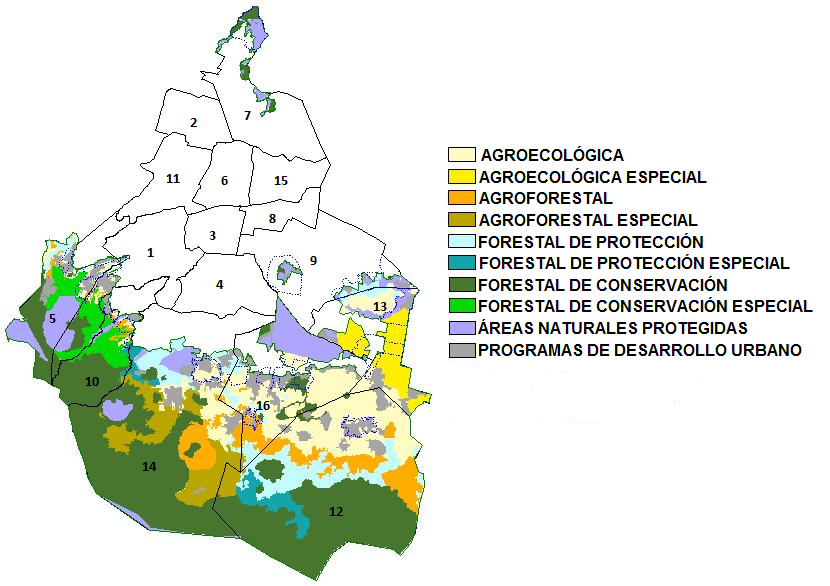
\includegraphics[width=100mm, scale=1]{ciudaddemexico}
  \caption{División política y uso de suelo en la Ciudad de México \citep{SEDEMA2016}}
  \label{ciudaddemexico}
\end{figure}

\newpage

El área de estudio contemplada en esta tesis se divide en 17 polígonos correspondientes a las 16 alcaldías de la Ciudad de México y el contorno de Ciudad Universitaria (campus principal de la UNAM) ubicada en la alcaldía Coyoacán, la cual es de especial interés debido a que alberga la Reserva Ecológica del Pedregal de San Ángel (REPSA).\\

La REPSA es una reserva natural de carácter urbano (no incluida en la categoría de suelo de conservación) protegida por la UNAM, lo cual garantiza un conocimiento ejemplar a través de las numerosas instituciones dedicadas a la investigación y divulgación científica. Su sustrato está conformado en su mayoría por roca basáltica la cual posee un alto valor biológico, ecológico y geomorfológico ya que permite recargar los mantos acuíferos, mantiene la humedad y la calidad del aire, y contribuye a amortiguar los cambios de temperatura en el microclima. La vegetación es de matorral xerófilo con marcada estacionalidad. Actualmente cuenta con una extensión de 237.33 hectáreas, que comprenden tres zonas núcleo y 13 zonas de amortiguamiento \citep{REPSA2019}.\\

En el Atlas de Riesgos de la REPSA \citep{AtlasREPSA} se cita la CL como una de las amenazas para los componentes biológicos del socioecosistema albergado por la REPSA y se menciona la necesidad de estudios en este sentido para la protección y conservación de la vida silvestre de Ciudad Universitaria.\\

La Ciudad de México está localizada en una zona sub-tropical donde las estaciones del año pueden ser separadas en tres periodos: Primavera Seca (PS) de abril a mayo, Temporada Lluviosa (TL) de junio a octubre e Invierno Seco (IS) de noviembre a marzo \citep{Jauregui2002}.\\

\subsection{Climatología de aerosol atmosférico y nubosidad}
\label{subsec:climatologia}

Para los fines de modelación de esta tesis resulta importante contar con la climatología de aerosol atmosférico y nubosidad en la Ciudad de México, como una referencia que permite realizar experimentos numéricos con condiciones cercanas a las reales.\\

\textbf{Aerosol atmosférico}

\cite{Carabali2017} realizaron la climatología de aerosol atmosférico para la Ciudad de México a partir de los datos obtenidos de 1999 a 2014 de la red AErosol RObotic NETwork (AERONET) para los periodos IS, PS y TL  (Tabla \ref{tab:climatologiaerosol}).\\

El AOD medido a 500 nm (AOD$_{500}$) provee una más robusta caracterización del AOD ya que a esa longitud de onda la absorción de vapor de agua y oxígeno es mínima \citep{Kanniah2009}. Por otro lado, el Parámetro de Angstrom calculado en el intervalo espectral 440-870 $(\alpha_{440-870})$ es el más adecuado para discriminar el tamaño de las partículas de aerosol atmosférico \citep{Kaskaoutis2007}.

\begin{table}[htb]
\centering
\caption{Climatología de aerosol atmosférico en la Ciudad de México \citep{Carabali2017}}
\label{tab:climatologiaerosol}
\resizebox{0.5\textwidth}{!}{%
\begin{tabular}{|c|c|c|}
\hline
\textbf{Periodo}        & \textbf{AOD$_{500}$} & \textbf{$\alpha_{440-870}$} \\ \hline
Invierno Seco (IS)      & 0.29         & 1.54           \\ \hline
Primavera Seca (PS)     & 0.33         & 1.49           \\ \hline
Temporada Lluviosa (TL) & 0.37         & 1.39           \\ \hline
\end{tabular}%
}
\end{table}

\newpage

\textbf{Nubosidad}

Aunque hasta la fecha no existe una climatología como tal de la nubosidad en la Ciudad de México, es posible inferir el tipo típico de nubes que se forman en cada uno de los periodos del año. Las nubes de interés para los experimentos numéricos de esta tesis son las nubes bajas y medias dada su cercanía en altitud con las fuentes artificiales de luz (Figura~\ref{nubes}).\\

A continuación se abordan las características de las nubes que forman parte del inventario del modelo \textit{SkyGlow} utilizado en este trabajo \citep{Cloudatlas1987}, \citep{Solano2015}.\\

\textit{\textbf{Altocumulus}}

\begin{itemize}

    \item Clasificación por altitud: nube media (3-5km)
    
    \item Formación: Generalmente a través de la condensación por ascenso de masas de aire húmedas
    
    \item Albedo espectral: 0.36 (350-800 nm)
    
\end{itemize}

\\

\textit{\textbf{Altostratus}}

\begin{itemize}

    \item Clasificación por altitud: nube media (3-5km)
    
    \item Formación: Asociadas a frentes (fríos, cálidos y ocluidos)
    
    \item Albedo espectral: 0.5 (350-800 nm)
    
\end{itemize}

\\

\textit{\textbf{Stratus}}

\begin{itemize}

    \item Clasificación por altitud: nube baja (700 m para este estudio)
    
    \item Formación: Condensación de masas de aire cálidas y húmedas en niveles bajos
    
    \item Albedo espectral: 0.5 (350-800 nm)
    
\end{itemize}

\\

\begin{figure}[htb]
  \centering
    \includegraphics[width=150mm, scale=1.5]{nubes}
  \caption{Nubes. A) Altocumulus, B) Altostratus, C) Stratus \citep{Metoffice2019}}
  \label{nubes}
\end{figure}

\newpage

\subsection{Consumo de energía eléctrica}
\label{subsec:consumoenergiaelectrica}

Con sólo 7\% de la población total de México, en la Ciudad de México se consume casi un tercio del petróleo demandado en el país y 6\% del total de la energía eléctrica \citep{SENER2013}. Las estadísticas muestran que del 100\% de energía eléctrica consumida en México, 30\% corresponde al sector residencial y de servicios públicos, sólo debajo del 52\% correspondiente a la industria \citep{Ramos2012}.\\

De acuerdo con el Sistema de Información Energética de la Secretaría de Energía, durante 2017 se consumieron en la Ciudad de México un total de 12,575,591 MW h$^{-1}$ de los cuales 2,938,559 MW h$^{-1}$ corresponden al sector residencial (23\%) de acuerdo con la Comisión Federal de Electricidad (Tabla \ref{tab:inventariocdmx}).\\

Es de interés conocer la relación entre el consumo de energía eléctrica y el cambio climático, lo cual es posible estimar a través de la emisión de Gases de Efecto Invernadero, más específicamente de CO$_{2}$ con el uso de la siguiente relación \citep{UTSEDEMA2018}: 

\begin{equation}
E_{CO_{2}} = W_{Elect}\: FE_{Elect}
\end{equation}

Donde $E_{CO_{2}}$ es la emisión en toneladas de CO$_{2}$ equivalente debida al consumo de energía eléctrica, $W_{Elect}$ es el consumo de energía eléctrica en MW h$^{-1}$ y $FE_{Elect}$ es el factor de consumo de energía eléctrica en toneladas de CO$_{2}$ equivalente por MW h$^{-1}$.\\

El factor de consumo de energía eléctrica se basa en el consumo total de combustible y la generación de electricidad neta entregada a la red. Varía cada año de acuerdo con la mezcla de combustibles empleados en la generación de electricidad distribuida por el Sistema Eléctrico Nacional, el cual está integrado por la Comisión Federal de Electricidad y productores independientes \citep{GEI2013}.\\

Considerando que el factor de consumo de energía eléctrica en 2017 fue 0.582 toneladas de CO$_{2}$ equivalente por MW h$^{-1}$ \citep{CRE2017}, se tiene que en 2017 se emitieron 7,318,993 toneladas de CO$_{2}$ por consumo de energía eléctrica en la Ciudad de México (6\% del total de las emisiones nacionales de CO$_{2}$ por consumo de energía eléctrica).\\

\subsection{Inventario de Alumbrado Público de la Ciudad de México}

Gracias a los datos brindados por las oficinas de transparencia de cada una de las alcaldías de la Ciudad de México y la Agencia de Gestión Urbana a través del Instituto de Transparencia, Acceso a la Información Pública, Protección de Datos Personales y Rendición de Cuentas de la Ciudad de México se construyó el \textbf{Inventario de Alumbrado Público de la Ciudad de México} (Tabla \ref{tab:inventariocdmx}).\\

Los datos de consumo de energía eléctrica por entidad federativa se obtuvieron a través del Sistema de Información Energética de la Secretaría de Energía (\url{sie.energia.gob.mx}}) y los datos de consumo de energía eléctrica por municipio producidos por la Comisión Federal de Electricidad se obtuvieron a través de la Plataforma Datos Abiertos del Gobierno de México (\url{datos.gob.mx}}).\\

\newpage

\begin{landscape}
\begin{table}[]
\centering
\caption{Inventario de Alumbrado Público de la Ciudad de México}
\label{tab:inventariocdmx}
\resizebox{1.4\textwidth}{!}{%
\begin{tabular}{llcccllcccc}
\hline
\multicolumn{1}{|c|}{\textbf{$\#$}} & \multicolumn{1}{c|}{\textbf{Alcaldía}} & \multicolumn{1}{l|}{\textbf{Extensión (km$^{2}$)}} & \multicolumn{1}{c|}{\textbf{\begin{tabular}[c]{@{}c@{}}Población\\ (número de habitantes)\end{tabular}}} & \multicolumn{1}{c|}{\textbf{Halogenuros metálicos ($\%$)}} & \multicolumn{1}{c|}{\textbf{LED ($\%$)}} & \multicolumn{1}{c|}{\textbf{\begin{tabular}[c]{@{}c@{}}Vapor de sodio de\\ alta presión ($\%$)\end{tabular}}} & \multicolumn{1}{c|}{\textbf{\begin{tabular}[c]{@{}c@{}}Número de luminarias\\ (vías primarias)\end{tabular}}} & \multicolumn{1}{c|}{\textbf{\begin{tabular}[c]{@{}c@{}}Número de luminarias\\ (vías secundarias)\end{tabular}}} & \multicolumn{1}{c|}{\textbf{\begin{tabular}[c]{@{}c@{}}Número de luminarias\\ (totales)\end{tabular}}} & \multicolumn{1}{c|}{\textbf{\begin{tabular}[c]{@{}c@{}}Consumo de energía eléctrica\\ sector residencial (MW h$^{-1}$)\end{tabular}}} \\ \hline
 &  & \multicolumn{1}{l}{} & \multicolumn{1}{l}{} & \multicolumn{1}{l}{} &  &  & \multicolumn{1}{l}{} & \multicolumn{1}{l}{} & \multicolumn{1}{l}{} & \multicolumn{1}{l}{} \\ \hline
\multicolumn{1}{|l|}{1} & \multicolumn{1}{l|}{Álvaro Obregón} & \multicolumn{1}{c|}{96.17} & \multicolumn{1}{c|}{749,982} & \multicolumn{1}{c|}{62} & \multicolumn{1}{c|}{} & \multicolumn{1}{c|}{38} & \multicolumn{1}{c|}{9,911} & \multicolumn{1}{c|}{71,397} & \multicolumn{1}{c|}{40,835} & \multicolumn{1}{c|}{210,903} \\ \hline
\multicolumn{1}{|l|}{2} & \multicolumn{1}{l|}{Azcapotzalco} & \multicolumn{1}{c|}{33.6} & \multicolumn{1}{c|}{400,161} & \multicolumn{1}{c|}{100} & \multicolumn{1}{l|}{} & \multicolumn{1}{c|}{} & \multicolumn{1}{c|}{5,009} & \multicolumn{1}{c|}{22,527} & \multicolumn{1}{c|}{27,536} & \multicolumn{1}{c|}{168,877} \\ \hline
\multicolumn{1}{|l|}{3} & \multicolumn{1}{l|}{Benito Juárez} & \multicolumn{1}{c|}{26.63} & \multicolumn{1}{c|}{417,416} & \multicolumn{1}{c|}{93} & \multicolumn{1}{c|}{7} & \multicolumn{1}{l|}{} & \multicolumn{1}{c|}{8,862} & \multicolumn{1}{c|}{27,550} & \multicolumn{1}{c|}{36,412} & \multicolumn{1}{c|}{234,458} \\ \hline
\multicolumn{1}{|l|}{4} & \multicolumn{1}{l|}{Coyoacán} & \multicolumn{1}{c|}{54.12} & \multicolumn{1}{c|}{608,479} & \multicolumn{1}{c|}{100} & \multicolumn{1}{l|}{} & \multicolumn{1}{l|}{} & \multicolumn{1}{c|}{6,463} & \multicolumn{1}{c|}{36,856} & \multicolumn{1}{c|}{43,319} & \multicolumn{1}{c|}{230,390} \\ \hline
\multicolumn{1}{|l|}{5} & \multicolumn{1}{l|}{Cuajimalpa de Morelos} & \multicolumn{1}{c|}{80.95} & \multicolumn{1}{c|}{199,224} & \multicolumn{1}{c|}{90} & \multicolumn{1}{l|}{} & \multicolumn{1}{c|}{10} & \multicolumn{1}{c|}{1,147} & \multicolumn{1}{c|}{13,186} & \multicolumn{1}{c|}{14,333} & \multicolumn{1}{c|}{72,127} \\ \hline
\multicolumn{1}{|l|}{6} & \multicolumn{1}{l|}{Cuauhtémoc} & \multicolumn{1}{c|}{32.44} & \multicolumn{1}{c|}{532,553} & \multicolumn{1}{c|}{100} & \multicolumn{1}{l|}{} & \multicolumn{1}{l|}{} & \multicolumn{1}{c|}{12,574} & \multicolumn{1}{c|}{26,938} & \multicolumn{1}{c|}{39,512} & \multicolumn{1}{c|}{286,460} \\ \hline
\multicolumn{1}{|l|}{7} & \multicolumn{1}{l|}{Gustavo A. Madero} & \multicolumn{1}{c|}{94.07} & \multicolumn{1}{c|}{1,164,477} & \multicolumn{1}{c|}{99} & \multicolumn{1}{c|}{1} & \multicolumn{1}{l|}{} & \multicolumn{1}{c|}{13,778} & \multicolumn{1}{c|}{46,362} & \multicolumn{1}{c|}{60,140} & \multicolumn{1}{c|}{415,940} \\ \hline
\multicolumn{1}{|l|}{8} & \multicolumn{1}{l|}{Iztacalco} & \multicolumn{1}{c|}{23.3} & \multicolumn{1}{c|}{390,348} & \multicolumn{1}{c|}{100} & \multicolumn{1}{l|}{} & \multicolumn{1}{l|}{} & \multicolumn{1}{c|}{6,056} & \multicolumn{1}{c|}{23,050} & \multicolumn{1}{c|}{29,106} & \multicolumn{1}{c|}{145,105} \\ \hline
\multicolumn{1}{|l|}{9} & \multicolumn{1}{l|}{Iztapalapa} & \multicolumn{1}{c|}{116.1} & \multicolumn{1}{c|}{1,827,868} & \multicolumn{1}{c|}{100} & \multicolumn{1}{l|}{} & \multicolumn{1}{l|}{} & \multicolumn{1}{c|}{12,700} & \multicolumn{1}{c|}{91,148} & \multicolumn{1}{c|}{103,848} & \multicolumn{1}{c|}{530,447} \\ \hline
\multicolumn{1}{|l|}{10} & \multicolumn{1}{l|}{Magdalena Contreras} & \multicolumn{1}{c|}{63.61} & \multicolumn{1}{c|}{243,886} & \multicolumn{1}{c|}{95} & \multicolumn{1}{c|}{5} & \multicolumn{1}{l|}{} & \multicolumn{1}{c|}{999} & \multicolumn{1}{c|}{9,200} & \multicolumn{1}{c|}{10,199} & \multicolumn{1}{c|}{44,762} \\ \hline
\multicolumn{1}{|l|}{11} & \multicolumn{1}{l|}{Miguel Hidalgo} & \multicolumn{1}{c|}{46.99} & \multicolumn{1}{c|}{364,439} & \multicolumn{1}{c|}{95} & \multicolumn{1}{c|}{5} & \multicolumn{1}{l|}{} & \multicolumn{1}{c|}{10,920} & \multicolumn{1}{c|}{30,838} & \multicolumn{1}{c|}{41,758} & \multicolumn{1}{c|}{185,013} \\ \hline
\multicolumn{1}{|l|}{12} & \multicolumn{1}{l|}{Milpa Alta} & \multicolumn{1}{c|}{228.4} & \multicolumn{1}{c|}{137,927} & \multicolumn{1}{c|}{100} & \multicolumn{1}{l|}{} & \multicolumn{1}{l|}{} & \multicolumn{1}{c|}{268} & \multicolumn{1}{c|}{10,226} & \multicolumn{1}{c|}{10,494} & \multicolumn{1}{c|}{20,645} \\ \hline
\multicolumn{1}{|l|}{13} & \multicolumn{1}{l|}{Tláhuac} & \multicolumn{1}{c|}{83.45} & \multicolumn{1}{c|}{361,593} & \multicolumn{1}{c|}{97} & \multicolumn{1}{c|}{3} & \multicolumn{1}{l|}{} & \multicolumn{1}{c|}{2,030} & \multicolumn{1}{c|}{18,389} & \multicolumn{1}{c|}{20,419} & \multicolumn{1}{c|}{90,984} \\ \hline
\multicolumn{1}{|l|}{14} & \multicolumn{1}{l|}{Tlalpan} & \multicolumn{1}{c|}{312} & \multicolumn{1}{c|}{677,104} & \multicolumn{1}{c|}{100} & \multicolumn{1}{l|}{} & \multicolumn{1}{l|}{} & \multicolumn{1}{c|}{5,313} & \multicolumn{1}{c|}{3,321} & \multicolumn{1}{c|}{8,634} & \multicolumn{1}{c|}{21,367} \\ \hline
\multicolumn{1}{|l|}{15} & \multicolumn{1}{l|}{Venustiano Carranza} & \multicolumn{1}{c|}{33.42} & \multicolumn{1}{c|}{427,263} & \multicolumn{1}{c|}{100} & \multicolumn{1}{l|}{} & \multicolumn{1}{l|}{} & \multicolumn{1}{c|}{9,970} & \multicolumn{1}{c|}{28,481} & \multicolumn{1}{c|}{38,451} & \multicolumn{1}{c|}{175,050} \\ \hline
\multicolumn{1}{|l|}{16} & \multicolumn{1}{l|}{Xochimilco} & \multicolumn{1}{c|}{122} & \multicolumn{1}{c|}{415,933} & \multicolumn{1}{c|}{95} & \multicolumn{1}{c|}{5} & \multicolumn{1}{l|}{} & \multicolumn{1}{c|}{1,488} & \multicolumn{1}{c|}{22,459} & \multicolumn{1}{c|}{23,947} & \multicolumn{1}{c|}{106,031} \\ \hline
 &  & \multicolumn{1}{l}{} & \multicolumn{1}{l}{} & \multicolumn{1}{l}{} &  &  & \multicolumn{1}{l}{} & \multicolumn{1}{l}{} & \multicolumn{1}{l}{} & \multicolumn{1}{l}{} \\ \cline{7-11} 
 &  & \multicolumn{1}{l}{} & \multicolumn{1}{l}{} & \multicolumn{1}{l}{} & \multicolumn{1}{l|}{} & \multicolumn{1}{c|}{\textbf{Total}} & \multicolumn{1}{c|}{107,488} & \multicolumn{1}{c|}{481,928} & \multicolumn{1}{c|}{589,416} & \multicolumn{1}{c|}{2,938,559} \\ \cline{7-11} 
\end{tabular}
}
\end{table}
\end{landscape}

\section{Hipótesis}

\vspace{5mm}

La cantidad, distribución y características de luz artificial producida por el alumbrado público da origen al brillo del cielo nocturno, que en mayor o menor medida, genera contaminación lumínica en las alcaldías de la Ciudad de México.\\

De manera general se considera que existe contaminación lumínica cuando los valores de radiancia son mayores al máximo valor natural registrado, es decir \textbf{10$^{-4}$ W sr$^{-1}$  m$^{-2}$} (véase \textbf{\autoref{subsec:componentesbrillocielo}}).\\

\section{Objetivos}

\vspace{5mm}

\subsection{Generales}

\vspace{5mm}

\begin{itemize}

	\item Estimar los niveles de contaminación lumínica en la Ciudad de México 

    \item Reproducir el modelo \textit{SkyGlow} para el caso de la Ciudad de México
    
    \item Generar un antecedente para la campaña de validación del modelo \textit{SkyGlow} en la Ciudad de México
    
\end{itemize}

\vspace{5mm}

\subsection{Particulares}

\begin{itemize}

    \item Elaborar el \textbf{Inventario de Alumbrado Público de la Ciudad de México}
    
    \item Generar el \textbf{Mapa Teórico de Contaminación Lumínica de la Ciudad de México} con salidas del modelo \textit{SkyGlow} 
    
    \item Comparar mediciones satelitales de radiancia contra los valores teóricos obtenidos con el modelo \textit{SkyGlow}
    
    \item Construir mediante experimentos numéricos con el modelo \textit{SkyGlow} diferentes escenarios del brillo del cielo nocturno tomando en cuenta diferentes posiciones del observador y condiciones atmosféricas
    
    \item Inferir la influencia del aerosol atmosférico  y la nubosidad en el brillo del cielo nocturno de la Ciudad de México a partir del objetivo anterior
    
    
\end{itemize}